\documentclass[mscThesis.tex]{subfiles}

\begin{document}

\chapter{Reinforcement Learning}
\label{chap:RL}
% Background
Reinforcement learning is a machine learning method, developed in the 1980's \cite{SuttonBarto1998}. The concept of RL is a combination of different methods in the field of artificial intelligence, adaptive- and optimal control. Reinforcement learning has successfully been applied in the field of artificial intelligence to teach computers to play chess and backgammon. In the field of control, reinforcement learning is a particular interesting method, but hard to realize in practice. The reason for this is that the state-space of robotics systems is continuous in multiple dimensions, compared to the finite state-space of chess. The search space for optimal solutions is therefore of a completely different order. Since the RL framework assumes no model of the system (some methods incorporate model learning), applying RL on a robotic system can be described as model-free, adaptive, optimal control. However, the representative power of the RL framework comes at a cost in lack of tractability properties.

% Purpose
In this Chapter we will outline the method of reinforcement learning as well as describe several reinforcement learning methods that are suitable for robotic applications. 

In Section \ref{sec:MDP}, a mathematical framework called the Markov Decision Process (MDP), which we will be using throughout is introduced. Several definitions that are used to describe the RL method, applied to robotic systems, are given as well. After that, in Section \ref{sec:RLMethods}, several main approaches of reinforcement learning are elaborated upon. We will finish the Chapter with a specific reinforcement learning method called black-box policy improvement ($\text{PI}^{BB}$), in Section \ref{sec:PIBB}. 

\section{Markov Decision Process}
\label{sec:MDP}

The RL framework considers an intelligent robot, called the agent, that has to do a task. In order to achieve the task, the agent can manipulate the environment by performing actions which will cause a transition to another state. Mathematically, the environment of the agent described above is called a Markov decision process. This process can be described as the following tuple: $(X, U, T)$ \cite{SuttonBarto1998}:

\begin{itemize}
\item $X$: A set of possible states that represent the dynamics of the system. It is assumed that the agent can sense the complete state.
\item $U$: A set of possible actions that the agent can select at each time step. 
\item $T$: The state transition probability function $T:X \times U \times X \rightarrow \mathbb{R}$. For each state $\bm{x} \in X$ the probability of transforming to the next state $\bm{x}' \in X$ by inferring action $\bm{u} \in U$ is given by $T(\bm{x},\bm{u},\bm{x}')$.
\end{itemize}

Note that the transition of the agent from state $\bm{x}$ to $\bm{x}'$ is not influenced by states prior to state $\bm{x}$. This is called the Markov property.

In this work we assume that all trajectories to have the same length in time. As such, we can define a trajectory $\bm{\tau}$ as the ordered set of state-action pairs from the initial state to the final state: $\bm{\tau} = \left\{ \left\{\bm{x}_0, \bm{u}_0, t_0 \right\}, ..., \left\{\bm{x}_N, \bm{u}_N, t_N \right\} \right\}$.

\subsection{Policy}
The policy, in some areas referred to as the control law, is the function $\pi:X \rightarrow U$ that makes the decision for control action. In discrete-state problems, the policy chooses an action $\bm{u}$ from a fixed set of actions. If the MDP is continuous, the control action is calculated. A policy can be a deterministic function but it can be a stochastic as well. Stochastic policies are commonly used in reinforcement learning because it forces the agent to move in unexplored areas in state-space. 

In continuous-time reinforcement learning problems, a common practice is to use parameterized policies. Let us denote vector $\bm{\theta}$ as the policy parameter. The function that maps such a policy from action $\bm{x}$ to the control action $\bm{u}$ would now also be dependent on the parameter vector $\bm{\theta}$ as such: $\bm{u} = \pi (\bm{x}, \bm{\theta})$.

The policy parameters allows us to directly change the policy. If the policy is a linear combination of the policy parameters, calculating the gradient of the policy with respect to the policy parameters is straight forward.     

\subsection{Reward}
The RL framework allows a variety of different reward functions, which capture the robotic task in a mathematical function. Whether or not a reward is given every time step depends on the task at hand. Reinforcement learning algorithms are designed to maximize the total accumulated reward, or \emph{return} per trajectory, as stated in Equation \eqref{eq:return}. 

\begin{equation}
\E \left[ R(\bm{\tau}) \right] = \E \left[ \sum_{ \left\{\bm{x}, \bm{u}, t \right\} \in \bm{\tau}} r(\bm{x}, \bm{u}, t) \right]
\label{eq:return}
\end{equation}

The expression for accumulated reward is very similar to the cost function used in optimal control algorithms, only difference being that the expression for accumulated reward should be maximized where as the cost function should be minimized. 


\subsection{Value function}
We continue by defining a useful definition for the accumulated reward that the agent obtains in time. The so-called value function or state-value function defines the expected return of an agent in state $\bm{x}$, when the optimal policy is used. 

\begin{equation*}
V( \bm{x})=\min_{\bm{u}_i : \bm{u}_N} \E \left[ \sum_{\bm{\tau}_{t_i} : \bm{\tau}_{t_N}} r( \bm{x}, \bm{u}, t ) \right]
\end{equation*}

\section{RL learning algorithms}
\label{sec:RLMethods}
The Markov decision process is a very powerful tool to create adaptive learning methods. Several algorithms are developed for MDPs over the years. In general, we can establish a common optimization problem that all RL methods solve in a different manner:

\begin{equation*}
\pi = \argmax_{\pi} \E \left[ R(\bm{\tau}) \right]
\end{equation*}

The group of reinforcement learning algorithms can roughly be divided into three main groups \cite{Babuska2012}: actor-only, actor-critic and critic-only methods, where the actor denotes the policy and the critic denotes the value function. 

\subsection{Critic-only methods}
In critic-only methods, the value function plays an important role. A critic-only algorithm consists of a method to learn the value function and a policy that chooses the control action in order to maximize this function. If the state-space and action-space of the MDP are finite, an approximation of the value for each state-action pair can be stored in computer memory. The values of each state-action pair can be updated using the temporal difference error. In that case, dynamic programming methods can be used as a policy. In continuous space the value function can be approximated. Also, discretizing a continuous state and action space is often done in critic-only algorithms. In critic-only methods, the value function can be updated either each time step or after each episode. Critic-only methods use an optimization algorithm in its policy. Each time step, the next control action is determined by optimizing the estimate of the value function. This is the basis for the Q-learning \cite{Watkins1989} and SARSA \cite{Rummery1994} algorithms. Critic-only methods tend to work very well in finite-space MDP problem such as playing back-gammon \cite{Tesauro1995}. In continuous state-space problems, such as robotics, critic-only methods are not often used. One of the main disadvantages of critic-only methods is its slow convergence speed.

\subsection{Actor-critic methods}
If both the value function and the policy function are learned by the agent we call the algorithm an actor-critic method. In these methods the critic is used to update current policy, prescribed by the actor, by evaluating the performance of the agent. 

In each iteration, two updates occur: one on the value function and one on the policy. In the first update step, the value function of the previous state is updated using the reward that followed. After that, the policy parameters are updated using the value function. In finite space MDPs the two updates can be performed after each time step, as shown in \cite{SuttonBarto1998}. A more practical approach for robotic applications is episodic natural actor critic method, which is designed for continuous state space. In this particular method, the update is calculated after sampling a batch of rollouts, a common feature in many robotic RL methods. 

\subsection{Actor-only methods}
Algorithms in the actor-only class of reinforcement learning are characterized by a policy learning algorithm. Typically, actor-only methods define the policy of the agent as a function with variable parameters, which can be tuned to optimize the expected return. 

Actor-only methods do not use the definition of value function such as critic-only methods, to learn which actions result in high returns. Instead, direct optimization over the definition of the expected return is common practice. A group of actor-only methods called gradient methods relies on optimizing the accumulated reward, by approximating the gradient of the expected return with respect to the policy parameters. An example of a known policy gradient method is REINFORCE \cite{williams1992}. One major drawback of this approach is that the policy gradient tends to have a high noise variance.

A second class of actor-only methods, called reward weighted average methods, circumvents the problem of gradient variance. This class of methods update the policy after performing multiple different trajectories, also called rollouts, on the robot. After each batch of rollouts, the algorithm will update the policy based on which rollouts turned out to have the highest return. This particular class of methods have shown to deal reasonable well in the high dimensional continuous space of robotic systems. Several methods of this type have been developed both originating from reinforcement learning, as well as the field of stochastic optimal control (see Figure \ref{fig:actor-critic}). Two main flavors of reward weighted average algorithms are relative entropy policy search \cite{peters2010reps} and path integral approaches \cite{Theodorou2010} (see Section \ref{sec:PIBB}). 
 
\begin{figure}
\centering
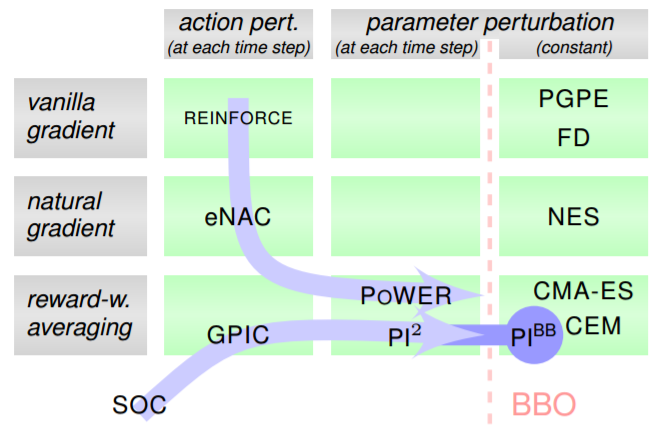
\includegraphics[width=0.5\textwidth, keepaspectratio=1]{figures/RLMethods.png}
\caption{Overview of RL methods commonly used in robotics \cite{Stulp2012}. The blue arrows indicates progress over time.}
\label{fig:actor-critic}
\end{figure} 

\section{Black box PI algorithm}
\label{sec:PIBB}
The specific algorithm that we will use is called black box policy improvement ($\text{PI}^{BB}$) \cite{Stulp2012}. This particular algorithm is suited to us for the following reason: The algorithm does not require a reward specified in each time step. Instead, the $\text{PI}^{BB}$ algorithm only requires the return over an update for each rollout. Learning a reward function for each part in state-space is much more difficult than learning the reward over complete trajectories, since the expert feedback will be given over complete or segmented trajectories, not for each state. 

\subsection{Episode based learning}
The $\text{PI}^{BB}$ algorithm is an episode based method. Each iteration $K$ number of episodes, also called rollouts will be run or simulated, resulting in multiple trajectories $\bm{\tau}_k$, where $k = 1,..., K$. After the sampling period, the return of each rollout is calculated and the new policy parameters $\bm{\theta}$ are calculated. This approach has proven to be more effective in robotics compared to traditional RL methods, in which an update is performed every time step. 

Another difference with traditional RL methods is the way reward weighted methods employ exploration noise. Exploration noise is added as a random vector to the parameters of the policy function: $\pi(\bm{\theta}+\bm{\epsilon_k})$. Where $\bm{\theta}$ is the parameter vector of the policy and $\bm{\epsilon}_k$, different for each rollout $k$, is a zero mean white noise vector with variance matrix $\matr{\Sigma}_{\epsilon}$. In order to regulate the exploration-exploitation trade-off, the variance of the exploration noise is decreased in a simulated annealing fashion.

\subsection{Reward weighting}
After sampling, the return of each trajectory will be calculated using the return function $R( \bm{\tau})$. This function can be a summation over a reward function $R( \bm{\tau}) = \sum_{\left\{ \bm{x},\bm{u},t \right\} \in \bm{\tau}} r(\bm{x}, \bm{u}, t)$ but this is not strictly necessary. 

Secondly, the probability for each rollout can be approximated using the return of each rollout in combination with the softmax operator. This can be achieved when using a batch of different rollouts. The probabilities that result from this approximation are relative with respect to the other rollouts in the batch.

\begin{gather*}
\tilde{S}(\bm{\tau}_k) = \frac{-h (R(\bm{\tau}_k) - \min_{\bm{\tau}_i \in \mathcal{T}} (R(\bm{\tau}_i)) )}{\max_{\bm{\tau}_i \in \mathcal{T}} (R(\bm{\tau}_i)) - \min_{\bm{\tau}_i \in \mathcal{T}} (R(\bm{\tau}_i)) )} \\
P(\bm{\tau}_{k}) = \frac{e^{-\tilde{S}(\bm{\tau}_k)}}{\sum_{\bm{\tau}_i \in \mathcal{T}} e^{\tilde{S}(\bm{\tau}_i)}}
\label{eq:PIBBProb}
\end{gather*}

We scaled the return of each trajectory relative to the minimum and maximum return obtained in batch $\mathcal{T}$. Also we changed from a return value $R$ to a cost measure $\tilde{S}$ in the first equation. Note that we scaled this scaled cost measure with $h$, a tuning parameter which determines how dense the probabilities of the different trajectories are distributed. We will use the probability of each rollout to formulate the policy update. Using the $\text{PI}^{BB}$ algorithm, optimizing the path integral comes down to a simple cost-weighted averaging function as described below. In Algorithm \ref{alg:PIBB}, the pseudo code of the $\text{PI}^{BB}$ algorithm is displayed.

\begin{gather*}
\delta \bm{\theta} = \sum_{\bm{\tau}_k \in \mathcal{T}} P(\bm{\tau}_k) \bm{\epsilon}_k \\
\bm{\theta} \gets \bm{\theta} + \delta \bm{\theta}
\end{gather*}


\begin{algorithm}
\caption{$\text{PI}^{BB}$ pseudo code}
\label{alg:PIBB}
\begin{algorithmic}[1]
\State initialize policy $\pi(\bm{x}, \bm{\theta}_0)$
\State initialize exploration noise and annealer $\Sigma_{\bm{\epsilon}}$, $\lambda$

\While{not converged}

\For{k = 1,...,K} 

\State Generate exploration noise 
\State $\bm{\epsilon}_k \sim  \mathcal{N} (0, \Sigma_{\bm{\epsilon}})$

\State Collect samples from the sample policy
\State $ \bm{\tau}_k = \left\{\bm{x}_i, \bm{u}_i = \pi (\bm{\theta}, \bm{\epsilon}_k) \right\}, i \in { 1, ... , N } $
\State $ \mathcal{T} = \{ \bm{\tau}_1, ..., \bm{\tau}_N \}$

\State Calculate reward
\State $R(\bm{\tau}_{k}) = \phi_{t_{N}} + \sum_{j=0}^{N-1} r_(\bm{x}_{t_{j}}, \bm{u}_{t_{j}}, t_{j})$

\EndFor

\State Calculate relative return
\State $\tilde{S}(\bm{\tau}_k) = \frac{-h (R(\bm{\tau}_k) - \min_{\bm{\tau}_i \in \mathcal{T}} (R(\bm{\tau}_i)) )}{\max_{\bm{\tau}_i \in \mathcal{T}} (R(\bm{\tau}_i)) - \min_{\bm{\tau}_i \in \mathcal{T}} (R(\bm{\tau}_i)) )}$

\State Calculate reward weighted probability
\State $P(\bm{\tau}_{k}) = \frac{e^{-\tilde{S}(\bm{\tau}_k)}}{\sum_{\bm{\tau}_i \in \mathcal{T}} e^{\tilde{S}(\bm{\tau}_i)}}$

\State Calculate policy update
\State $\delta \bm{\theta} = \sum_{\bm{\tau}_k \in \mathcal{T}} P(\bm{\tau}_k) \bm{\epsilon}_k$
\State $\bm{\theta} \gets \bm{\theta} + \delta \bm{\theta}$

\State Apply noise annealing 
\State $\matr{\Sigma}_{\epsilon} = \lambda \matr{\Sigma}_{\epsilon}$ 

\EndWhile
\end{algorithmic}
\end{algorithm}

\clearpage

% Bibliography
%\bibliographystyle{ieeetr}
%\printbib{bibliography}
%

\end{document}